% !TEX program = XeLaTeX
% !BIB program = bibtex
\documentclass[12pt, a4paper, oneside]{book}
\usepackage{amsmath}
\usepackage{amssymb}
\usepackage{amsthm}
\usepackage{graphicx}
\usepackage{latexsym}
\usepackage{pslatex}
\usepackage{color}
\usepackage{cite}
\usepackage{indentfirst}
\usepackage{tocloft}
\usepackage{multirow}
\usepackage{fontspec}

% Times New Roman
\setromanfont[
BoldFont=Times New Roman Bold.ttf,
ItalicFont=Times New Roman Italic.ttf,
BoldItalicFont=Times New Roman Bold Italic.ttf,
]{Times New Roman.ttf}
%\setmainfont{Times New Roman}

% Centering Chapter
\usepackage{sectsty}
\chapterfont{\centering}

\pagestyle{myheadings}
\setlength{\parindent}{0.8in}

\usepackage[top=1.5in,bottom=1in,left=1.5in,right=1in]{geometry}

\theoremstyle{plain}
\newtheorem{thm}{Theorem}[chapter]
\newtheorem{lem}[thm]{Lemma}
\newtheorem{cor}[thm]{Corollary}
\newtheorem{prop}[thm]{Proposition}
\newtheorem{rem}[thm]{Remark}
\newtheorem{ex}[thm]{Example}
\newtheorem{de}[thm]{Definition}
\renewcommand{\proof}{\textbf{Proof.}}

\numberwithin{equation}{chapter} \DeclareMathOperator{\Var}{var}
\DeclareMathOperator{\Ima}{Im}

\usepackage{float}
%\usepackage[skip=2pt,font=footnotesize]{caption}

\usepackage{graphics,graphicx}
\usepackage{calc}
\usepackage{tikz}
\usetikzlibrary{decorations.markings}
\tikzstyle{vertex}=[circle, draw, inner sep=2pt, minimum size=4pt]
\newcommand{\vertex}{\node[vertex]}
\newcounter{Angle}

\renewcommand{\baselinestretch}{1.5}

\newcommand*{\QEDA}{\hfill\ensuremath{\large{\lozenge}}}
\newcommand*{\QEDAa}{\hfill\ensuremath{\square}}

\renewcommand{\bibname}{\centerline{\Large REFERENCES}}

\usepackage{tocloft}
\renewcommand{\contentsname}{\hfill\bfseries\Large TABLE OF CONTENTS \hfill}
\renewcommand{\cftaftertoctitle}{\hfill}

\renewcommand{\listtablename}{\hfill\bfseries\Large LIST OF TABLES}
\renewcommand{\cftafterloftitle}{\hfill}

\renewcommand{\listfigurename}{\hfill\bfseries\Large LIST OF FIGURES}
\renewcommand{\cftafterloftitle}{\hfill}



\renewcommand{\cftchapleader}{\cftdotfill{\cftdotsep}}
\renewcommand{\cftsecleader}{\cftdotfill{\cftdotsep}}
\renewcommand{\cftsubsecleader}{\cftdotfill{\cftdotsep}}
\renewcommand{\contentsname}{Mục lục}
\renewcommand{\chaptername}{Chương}

\usepackage{titlesec}
\titleformat{\chapter}[block]{\centering\normalfont\huge\bfseries}{\chaptername~\thechapter.}{0.5em}{}

\graphicspath{{assets/}}

\usepackage{listings}

\usepackage[colorlinks=true, linkcolor=black]{hyperref}


\definecolor{codegreen}{rgb}{0,0.6,0}
\definecolor{codegray}{rgb}{0.5,0.5,0.5}
\definecolor{codepurple}{rgb}{0.58,0,0.82}
\definecolor{backcolour}{rgb}{0.95,0.95,0.92}

% Cấu hình style chung cho listings
\lstset{
    backgroundcolor=\color{backcolour},   % Màu nền
    commentstyle=\color{codegreen},       % Màu chú thích (comment)
    keywordstyle=\color{magenta},         % Màu từ khóa (keyword)
    numberstyle=\tiny\color{codegray},    % Style cho số dòng
    stringstyle=\color{codepurple},       % Màu cho chuỗi (string)
    basicstyle=\ttfamily\footnotesize,    % Font chữ monospace, size nhỏ
    breakatwhitespace=false,         
    breaklines=true,                      % Tự động xuống dòng nếu code quá dài
    captionpos=b,                         % Vị trí caption (b = bottom)
    keepspaces=true,                 
    numbers=left,                         % Đánh số dòng ở bên trái
    numbersep=5pt,                        % Khoảng cách từ số dòng đến code
    showspaces=false,                
    showstringspaces=false,
    showtabs=false,                  
    tabsize=4,                            % Độ rộng của Tab
    frame=single                          % Đóng khung viền xung quanh code
}

\usepackage{hyperref}
\usepackage{tabularx}

\begin{document}
% --- Trang bìa ---
\thispagestyle{empty}
\begin{center}
    \begin{figure}[h!]
    \centering
    
\includegraphics[width = 7.0cm]{HCMCOU_Logo.png}
    \end{figure}

    {\fontsize{30pt}{25pt}\selectfont\bfseries
    FACE DETECTION WITH RETINAFACE\par}
    \vspace{2.0cm} 

    {\fontsize{20pt}{25pt}\selectfont\bfseries
    ĐỒ ÁN MÔN HỌC\par}
    \vspace{0.25cm}
    {\fontsize{15pt}{25pt}\selectfont\bfseries
    Môn: Máy học\par}
    \vspace{5.0cm}
    
    {\fontsize{20pt}{15pt}\selectfont\bfseries
    TP. HỒ CHÍ MINH, 2026}
\end{center}

\newpage
\thispagestyle{empty}
\begin{center}
    \begin{figure}[h!]
    \centering
    
\includegraphics[width = 7.0cm]{HCMCOU_Logo.png}
    \end{figure}

    {\fontsize{25pt}{20pt}\selectfont\bfseries NHÓM 6\par}
    \vspace{1.5cm}
    {\large \textbf{THÀNH VIÊN}}\\
    \vspace{0.3cm}
    {\large
    \begin{tabular}{r c l}
        \textbf{2351010176} & \textbf{-} & \textbf{Phạm Minh Quân} \\
        \textbf{2351010238} & \textbf{-} & \textbf{Lê Khắc Tùng} \\
        \textbf{2351010227} & \textbf{-} & \textbf{Phạm Quý Trưởng} \\
        \textbf{2351010242} & \textbf{-} & \textbf{Nguyễn Bảo Việt} \\
        \textbf{2351010228} & \textbf{-} & \textbf{Hoàng Việt Tuấn} \\
    \end{tabular}}
    \vspace{2.0cm}

    {\fontsize{17pt}{15pt}\selectfont\bfseries
    Giáo viên hướng dẫn: LÊ VIẾT TUẤN}
    \vspace{3.0cm}

    {\fontsize{20pt}{15pt}\selectfont\bfseries
    TP. HỒ CHÍ MINH, 2026}
\end{center}

% --- Mục lục ---
\newpage
\pagenumbering{roman} 
\tableofcontents
\newpage

% --- NỘI DUNG ---
\pagenumbering{arabic} 
\setcounter{page}{1}
\pagestyle{myheadings}

\chapter{Giới thiệu}
\section{Tổng quan paper: }
\begin{itemize}
    \item[--] Bài toán nhận diện khuôn mặt đã trở thành một trong những bài toán kinh điển trong lĩnh vực \textbf{AI for Computer Vision}
    \item[--] Mặc dù có những bước tiến vượt bậc trong việc phát hiện \textbf{uncontrolled face} -- phát hiện được những khuôn mặt trong những thách thức về không gian như ánh sáng, pose hay những góc khuất, việc định vị chính xác và hiệu quả khuôn mặt trong môi trường thực tế vẫn đang là thách thức lớn chưa được giải quyết triệt để. 
    \item[--] RetinaFace -- Single-stage face detector, được giới thiệu là một giải pháp mạnh mẽ trong việc phát hiện từng \textbf{pixel-wise} (điểm ảnh) trên nhiều tỉ lệ khuôn mặt khác nhau bằng cách tận dụng lợi thế của \textbf{extra-supervised} và \textbf{self-supervised multi-task learning}.
\end{itemize}

\subsection{Extra-supervised Learning -- Học có giám sát bổ sung:}
\begin{itemize}
    \item[--] Trong Supervised Learning, mô hình được huấn luyện dựa trên bộ dữ liệu có label.
    \item[--] Trong Extra-supervised Learning, ngoài label có sẵn, ta \textbf{cung cấp thêm} cho mô hình các \textbf{auxiliary labels (nhãn phụ trợ)} chi tiết hơn ở một khía cạnh khác so với label của tác vụ chính.
    \item[--] Mục đích:
    \begin{itemize}
        \item[+] Giảm Overfitting: Việc phải dự đoán đúng nhiều loại label cùng lúc giúp mô hình học được các đặc trưng tổng quát hơn, thay vì chỉ học vẹt một tác vụ duy nhất.
        \item[+] Giúp mô hình chú ý đến các chi tiết quan trọng của dữ liệu mà nếu chỉ sử dụng 1 label chính, mô hình có thể bỏ qua.
    \end{itemize}
\end{itemize}
\subsection{Self-supervised Multi-task Learning -- Học đa tác vụ tự giám sát:}
\begin{itemize}
    \item[--] \textbf{Self-supervised learning (Học tự giám sát):} Là phương pháp học mà mô hình tự tạo ra label từ dữ liệu gốc mà không cần gán label thủ công.
    \item[--] \textbf{Multi-task learning (Học đa tác vụ):} Là phương pháp thiết kế một neural network duy nhất để giải quyết nhiều bài toán khác nhau cùng một lúc (chia sẻ chung các layer trích xuất đặc trưng đầu vào).
    \item[--] \textbf{Self-supervised Multi-task Learning: } Là mô hình học song song nhiều tác vụ cùng một lúc, trong đó có ít nhất một tác vụ tự tạo ra nhãn từ input.
    \item[--] Mục đích:
    \begin{itemize}
        \item[+] Tận dụng tối đã dữ liệu chưa gán nhãn: Cho phép mô hình học các biểu diễn hình học, cấu trúc hoặc ngữ cảnh thông qua nhánh self-supervised, từ đó hỗ trợ tăng cường độ chính xác cho các nhánh học có giám sát khác.
    \end{itemize}     
\end{itemize}

\section{WIDER FACE Dataset:}
\begin{itemize}
    \item[--] RetinaFace sử dụng \textbf{WIDER FACE} dataset -- \textbf{Face Detection Benchmark} \cite{yang2016wider}.
    \item[--] Bộ dataset này chứa nhiều annotations khác nhau bao gồm: Occlusions (độ che khuất), poses, event categories, face bounding boxes...
    \item[--] WIDER FACE bao gồm 32,203 ảnh và 393,703 face bounding boxes với mức độ biến đổi cao về scale, poses, expression, occlusion và illumination.
    \item[--] WIDER FACE được chia thành 40\% training, 10\% validation và 50\% testing bằng cách \textbf{randomly sampling} (Lấy mẫu ngẫu nhiên) từ 61 scene categories.
    \item[--] Dựa vào tỷ lệ phát hiện của thuật toán EdgeBox, khuôn mặt được phân thành 3 levels: Easy, Medium và Hard thông qua việc bổ sung dần các mẫu khó. 
    \item[--] \textbf{Extra Annotations.} Nhóm tác giả paper đã xác định được 5 cấp độ chất lượng hình ảnh khuôn mặt (levels of face image quality) và tiến hành gán nhãn thủ công, bổ sung 5 điểm mốc khuôn mặt (facial landmarks) bao gồm: tâm 2 mắt, chóp mũi và 2 khóe miệng. 
    \begin{figure}[h!]
        \centering
        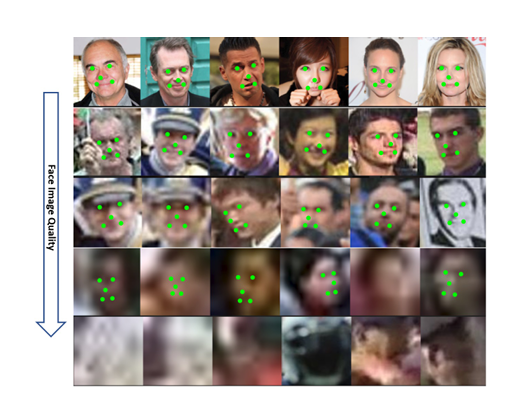
\includegraphics[width=0.8\textwidth]{extra_annotations.png}
        \caption{Các extra annotations của 5 facial landmarks}
    \end{figure}
    \item[--] Tổng cộng đã gán nhãn 84,600 faces trên training set và 18,500 faces trên validation set
\end{itemize}


\chapter{Metrics và Box trong Face Detection}
\section{Bounding Box:}
\begin{itemize}
    \item[--] Bounding box là phần khung bao quanh 1 object.
    \item[--] \textbf{Các chuẩn biểu diễn tọa độ phổ biến: }
        \item[+] Min max: $(x_{min}, y_{min}, x_{max}, y_{max})$   
        \item[+] Center-Size: $(x_{center}, y_{center}, width, height)$ 
    \vspace{0.2cm}
    \begin{figure}[h!]
        \centering
        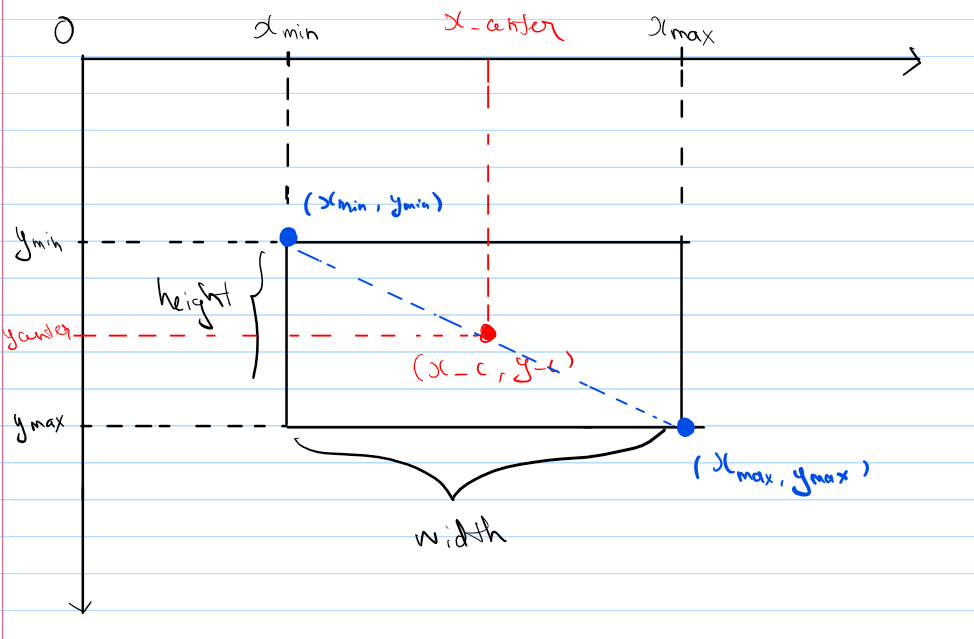
\includegraphics[width=0.8\textwidth]{coordinate.png}
        \caption{Hệ trục tọa độ của các điểm trên}
    \end{figure}
\end{itemize}


\section{WIDERFACE Annotations:}
\begin{itemize}
    \item[--] \textbf{Cấu trúc annotations} trong label.txt mà paper cung cấp:
        \item[+] File name
        \item[+] Number of bounding Box
        \item[+] \(x_1\), \(y_1\), w, h, blur, expression, illumination, invalid, occlusion, pose
\end{itemize}

\section{Jaccard:}
\begin{itemize}
    \item[--] \textbf{Jaccard Index (Hệ số tương đồng Jaccard)} -- là một con số dùng để đo lường mức độ tương đồng giữa hai tập hợp dữ liệu trong xác suất thống kê (statistic)
    \[J(A,B) = \frac{|A \cap B|}{|A \cup B|} = \frac{|A \cap B|}{|A| + |B| - |A \cap B|}\]
\end{itemize}

\section{Intersection over Union (IoU):}
\begin{itemize}
    \item[--] \textbf{IoU} là một metric dùng để đánh giá mức độ trùng lấp (overlap) giữa 2 bounding boxes.
    \item[--] Công thức tổng quát:
    \[\textbf{IoU} = \frac{\textbf{Area of Intersection}}{\textbf{Area of Union}}\] 
    
    \begin{figure}[H]
        \centering
        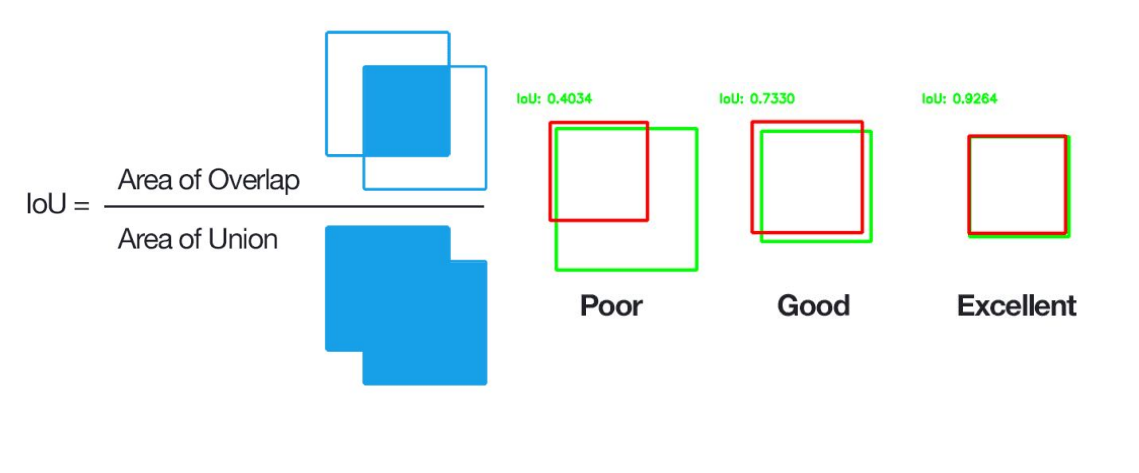
\includegraphics[width=0.8\textwidth]{IoU.png}
        \caption{Minh họa IoU}
    \end{figure}

    \subitem \textbf{Intersection:} Phần giao giữa hai bounding boxes
    \subitem \textbf{Union:} Phần hợp giữa hai bounding boxes
    \item[--] Hai bounding boxes càng overlap nhau, IoU càng \textbf{gần 1}, độ chính xác càng cao, object được detect càng tốt.
    \item[--] Hai bounding boxes càng lệch nhau, IoU càng \textbf{gần 0}, độ chính xác càng giảm, object detect sai 
\end{itemize}

\section{Average Precision và Mean Average Precision:}
\subsection{Average Precision (AP):}
\begin{itemize}
    \item[--] AP dùng để đo độ chính xác của mô hình cho một class duy nhất.
    \item[--] Cách tính:
    \begin{enumerate}
        \item[+] Liệt kê tất cả các bounding boxes mà mô hình dự đoán được, sắp xếp giảm dần dựa vào \textbf{confidence score}
        \item[+] So sánh với ground truth bằng IoU qua threshold (Ngưỡng), thường là 0.5.
        \begin{itemize}
            \item[.] \textbf{True Positive (TP):} Dự đoán có IoU \(\ge\) threshold với Ground Truth
            \item[.] \textbf{False Positive (FP):} Dự đoán có IoU < threshold với Ground Truth
            \item[.] \textbf{False Negative {FN}:} Ground truth mà mô hình bỏ lỡ (không detect được)
        \end{itemize}
        \item[+] Tính Precision và Recall:
        \[Precision = \frac{TP}{TP + FP}\ \quad ; \quad Recall = \frac{TP}{TP + FN}\]
        \item[+] Vẽ Precision-Recall Curve:
        \begin{figure}[H]
            \centering
            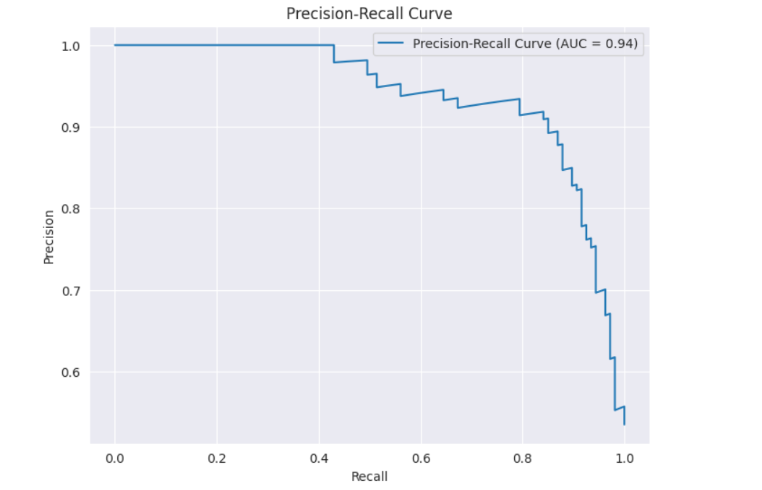
\includegraphics[width=0.7\textwidth]{precision_recall_curve.png}
            \caption{Minh họa Precision-Recall Curve}
        \end{figure}
        \item[+] AP = diện tích dưới đường Precision-Recall (Area under the precision-recall curve AUC-PR)
        \item[+] Công thức tổng quát:
        \[AUCPR = \int_{0}^1 P(R) \, dR\]
        \begin{itemize}
            \item[.] \(P(R)\): precision tại recall R
        \end{itemize} 
        \item[+] Công thức rời rạc:
        \[AUCPR = \sum_{n} (R_n - R_{n-1}) P_n\]
        \begin{itemize}
            \item[.] \(P_n\): Precision tại điểm n
            \item[.] \(R_n\): Recall tại điểm n
            \item[.] \(R_n - R_{n-1}\): Độ tăng recall (\(R_n\) và \(R_{n-1}\) là các mức Recall kế tiếp nhau sau khi đã sắp xếp theo Confidence Score)
        \end{itemize}
    \end{enumerate}    
\end{itemize}
\subsection{Mean Average Precision (mAP):}
\begin{itemize}
    \item[--] mAP là trung bình giá trị AP của tất cả classes.
    \[mAP = \frac{1}{N}\sum_{i=1}^{N}A{P_i}\]
    \begin{itemize}
        \item[+] \(N\): Số lượng classes.
        \item[+] \(A{P_i}\): giá trị AP tại class thứ i.
    \end{itemize}

\end{itemize}

\chapter{Related works}
\section{Image Pyramid và Feature Pyramid:}
Image Pyramid và Feature Pyramid là hai phương pháp được sử dụng để giải quyết thách thức về sự thay đổi tỷ lệ (scale) kích thước khuôn mặt.
\subsection{Image Pyramid}
\begin{itemize}
    \item[--] Mô hình dựa trên cơ chế sliding-windows, trong đó classifier sẽ được quét qua một lưới hình ảnh dày đặc (dense image grid)
\end{itemize}
\subsection{Feature Pyramid}
\begin{itemize}
    \item[--] Mô hình được xây dựng dựa trên \textbf{Image Pyramid}, kết hợp giữa sliding-anchor (cơ chế mỏ neo trượt) trên multi-scale feature maps đã thống trị \textbf{(dominated)} trong lĩnh vực face detection.
\end{itemize}
\begin{figure}[H]
    \centering
    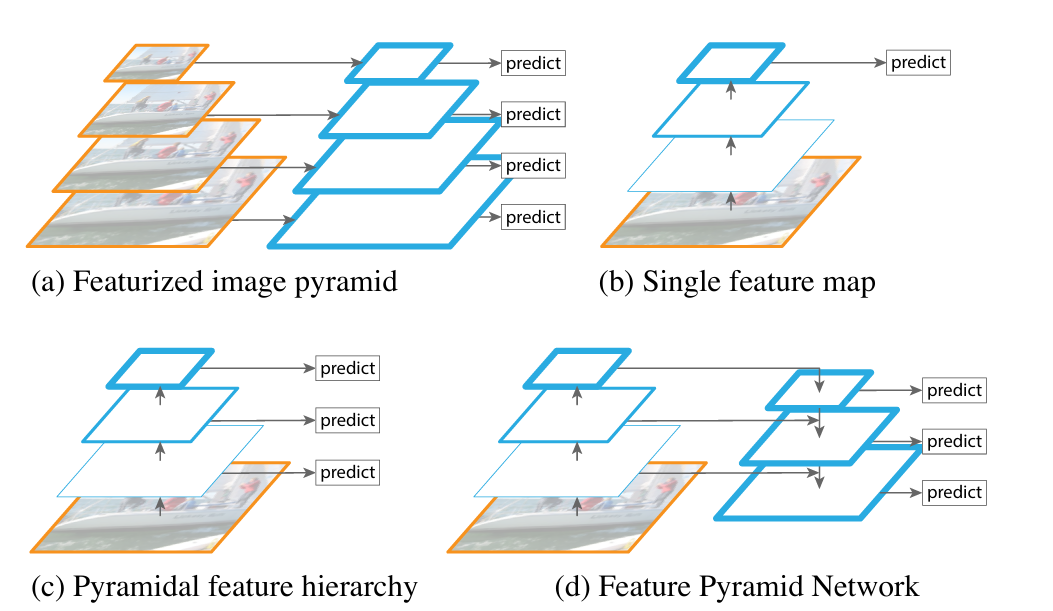
\includegraphics[width=1\textwidth]{pyramid.png}
    \caption{Minh họa Feature Pyramid được xây dựng dựa trên Image Pyramid}
\end{figure}

\section{Two-stage và Single-stage:}
\subsection{Two-stage:}
\begin{itemize}
    \item[--] \textbf{Giai đoạn 1 - Đề xuất vùng (Region Proposal Generation):} Sử dụng các thuật toán như Selective Search hoặc Region Proposal Network (RPN) trong các kiến trúc hiện đại (Faster R-CNN) để xác định các vùng ứng viên có khả năng chứa object.
    \item[--] \textbf{Giai đoạn 2 - Phân loại và Tinh chỉnh (Classification \& Regression):} Với mỗi Region Proposal, mô hình thực hiện đồng thời hai nhiệm vụ:
    \begin{itemize}
        \item \textit{Phân loại đối tượng (Object Classification):} Phân loại đối tượng trong region proposal thuộc class nào.
        \item \textit{Hồi quy khung hình (Bounding Box Regression):} Tính toán các độ sai lệch (offsets) để điều chỉnh tọa độ của vùng đề xuất ban đầu sao cho (fit) object nhất.
    \end{itemize}
\end{itemize}
\subsection{Single-stage:}
\begin{itemize}
    \item[--] Object Classification và Bounding Box Regression được thực hiện trực tiếp trên toàn bộ image mà không cần qua Region Proposal Generation.
    \item[--] RetinaFace là mô hình kiến trúc Single-Stage.
\end{itemize}
\begin{figure}[H]
    \makebox[\textwidth][c]{
        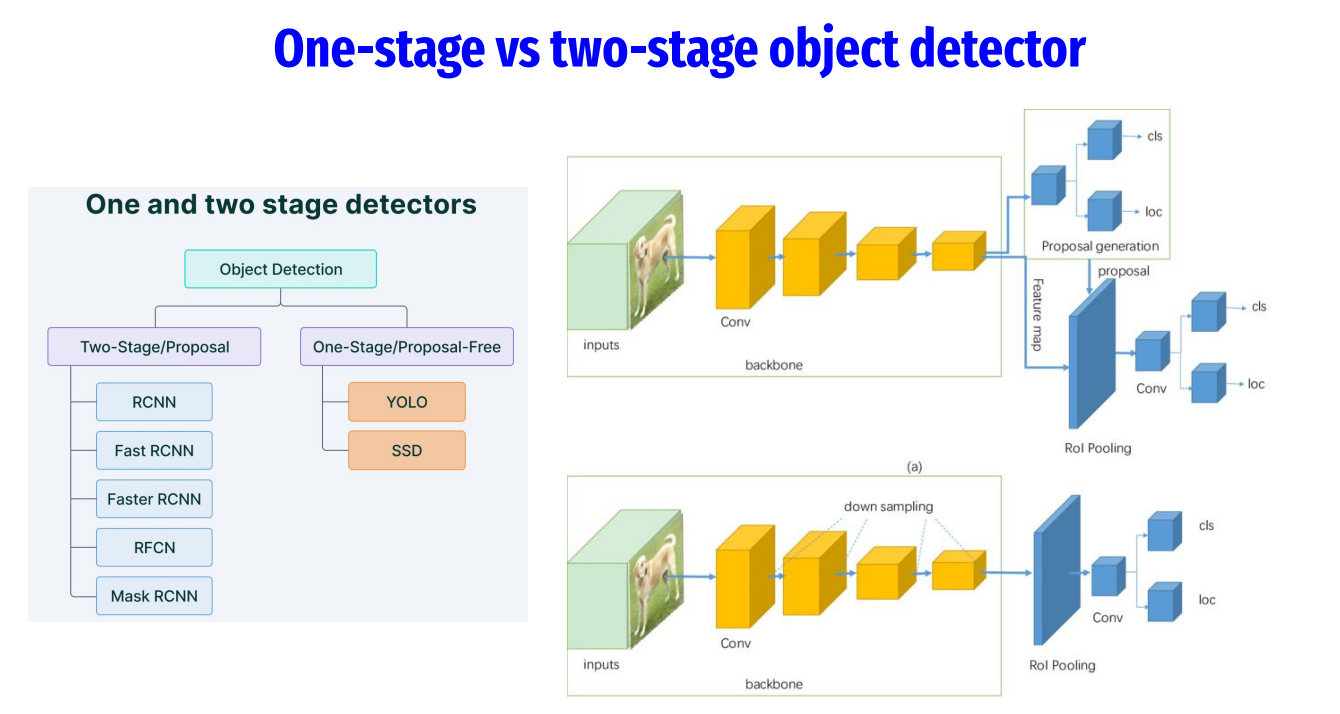
\includegraphics[width=1.28\textwidth]{object_detector.png}
    }
    \caption{Minh họa Single-stage và Two-stage Object Detector}
\end{figure}


\section{Context Modelling:  \eqref{eq:context_modules}}
\begin{itemize}
    \item[--] Context Modelling là một kỹ thuật để tăng cường khả năng suy luận ngữ cảnh của neural network, đặc biệt nhằm mục đích phát hiện các khuôn mặt cực kỳ nhỏ (tiny face).
    \item[--] Trong RetinaFace, để tăng cường khả năng capturing tiny faces, SSH \textbf{(Single Stage Headless) - Module for feature extraction} và PyramidBox đã áp dụng context modules trên feature pyramid để mở rộng receptive field từ Euclidean grids.
    \item[--] Để tăng cường non-rigid transformation modelling, RetinaFace sử dụng \textbf{Deformable Convolution Network (DCN)} \cite{dai2017deformable} để thay thế toàn bộ 3 x 3 convolution layers bên trong lateral connections cũng như bên trong chính các context modelling.
\end{itemize}
\section{Multi-task Learning}
\begin{itemize}
    \item[--] Là cách học mà một mô hình có thể giải quyết được nhiều tasks khác nhau
    \item[--] Trong RetinaFace, Multi-task Learning là chiến lược thiết kế một neural network duy nhất để giải quyết đồng thời nhiều bài toán face detection khác nhau từ cùng một input image, giúp các bài toán chia sẻ feature extraction và bổ trợ chéo cho nhau.
    \item[--] Cấu trúc Multitask-Learning trong RetinaFace: sử dụng một lớp tính toán dùng chung (shared loss head với 1 x 1 convolution layer) áp dụng lên các tầng của feature pyramid. Với mỗi positive anchor, network sẽ dự đoán đồng thời 4 thông tin:
    \begin{itemize}
        \item[+] Face score
        \item[+] Face box 
        \item[+] 5 facial landmarks
        \item[+] Dense 3D face vertices: Cấu trúc 3D dày đặc của khuôn mặt được chiếu lên image plane (self-supervised Learning).  
    \end{itemize}  
    \begin{figure}[H]
        \makebox[\textwidth][c]{
        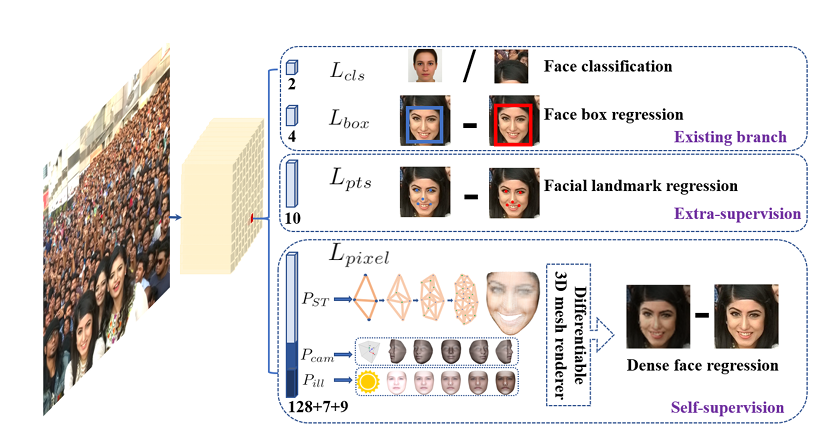
\includegraphics[width=1.20\textwidth]{multitask.png}}
        \caption{Phương pháp single-stage pixel-wise được đề xuất bằng cách sử dụng extra-supervised và self-supervised multi-task learning song song với các box classification và regression branches hiện có. Mỗi positive anchor bao gồm: (1) face score, (2) face box, (3) 5 facial landmarks, (4) dense 3D face vertices được chiếu trên image plane}
    \end{figure}
\end{itemize}
\chapter{RetinaFace Architecture}
\section{Thông tin chung:}
\subsection{Multi-task Loss:}
\begin{itemize}
    \item[--] Với mỗi training anchor \(i\), ta sẽ minimise multi-task loss có công thức:
    \begin{equation}
    L = L_{cls}(p_i,p_i^*) + \lambda_1p_i^*L_{box}(t_i,t_i^*) + \lambda_2p_i^*L_{pts}(l_i,l_i^*) + \lambda_3p_i^*L_{pixel}. \tag{1}
    \end{equation}
    \item[--](1) Face classification loss \(L_{cls}(p_i,p_i^*)\): Là \textbf{Softmax loss for binary classes (face/not face)} dùng để tính xác suất \(p_i\) xem anchor thứ i có phải là face hay không, \(p_i^*\) = 1 nếu positive anchor (có chứa face) và 0 nếu negative anchor
    \item[--](2) Face box regression loss \(L_{box}(t_i,t_i^*)\) Là regression loss:
    \begin{itemize}
        \item[+] Với \(t_i = \{t_x, t_y, t_w, t_h\}_i\) và \(t_i^* = \{t_x^*, t_y^*, t_w^*, t_h^*\}_i\) lần lượt là tọa độ (coordinates) của predicted box và grouth truth box liên quan đến positive anchor \((p_i^* = 1)\)
        \item[+] Paper tuân thủ theo \cite{girshick2015fast} để normalise box regression targets (centre location, width, height) và \(L_{box}(t_i,t_i^*) = R(t_i - t_i^*)\) với \(R\) là robust loss function (smooth-L1) được định nghĩa trong \cite{girshick2015fast}.
    \end{itemize}
    \begin{equation}
    Smooth_{L1}(x) = 
        \begin{cases}
            0.5x^2  & \text{if } |x| < 1 \\ 
            |x| - 0.5 & \text{otherwise,} 
        \end{cases} \tag{1.1}
    \end{equation}
    \item[--](3) Facial landmark regression Loss \(L_{pts}(l_i,l_i^*)\)
    \begin{itemize}
        \item[+] Với \(l_i = \{l_{x_1}, l_{y_1}, \dots, l_{x_5}, l_{y_5}\}_i\) và \(l_i = \{l_{x_1}^*, l_{y_1}^*, \dots, l_{x_5}^*, l_{y_5}^*\}_i\) lần lượt là predicted 5 facial landmarks và grouth truth liên quan đến positive anchor.
        \item[+] Tương tự box centre regression, 5 facial landmark regression cũng sử dụng target normalisation dựa trên anchor centre. 
    \end{itemize}
    \item[--](4) Dense regression loss \(L_{pixel}\) (tham chiếu mục \eqref{eq:pixel_loss})
    \item[--] Loss-balancing parameters \(\lambda_1-\lambda_3\) được gán giá trị lần lượt là 0.25, 0.1 và 0.1. Có nghĩa là ta tăng đáng kể tầm quan trọng của box và landmark locations từ supervision signals.
\end{itemize} 
\subsection{Dense Regression Branch:}
\label{eq:pixel_loss}
\begin{itemize}
    \item [--]\textbf{Mesh Decoder:} paper đã employ trực tiếp mesh decoder (mesh convolution và mesh up-sampling) từ \cite{zhou2019dense,ranjan2018generating}.
    \begin{itemize}
        \item [+] Thay vì sử dụng convolution 2D thông thường (tính toán trên lưới không gian Euclid), nhánh này sử dụng \textbf{Graph Convolution} (tích chập đồ thị) để thao tác với các đỉnh trên mô hình lưới 3D.
        \item [+] Mesh decoder thực hiện dự đoán đồng thời cả shape và texture của face thông qua phương pháp fast localised spectral filtering (lọc quang phổ cục bộ nhanh).
    \begin{figure}[H]
        \makebox[\textwidth][c]{
            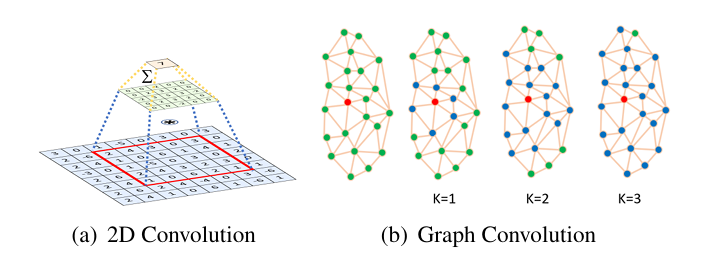
\includegraphics[width=1.0\textwidth]{convolution.png}}
            \caption{Minh họa 2D Convolution trong không gian lưới Euclid và Graph Convolution}
    \end{figure}
    \begin{itemize}
    \item \textbf{(a) 2D Convolution} là một \textit{kernel-weighted neighbour sum} bên trong lưới Euclid receptive field. Mỗi lớp tích chập (\textit{convolutional layer}) chứa \( \text{Kernel}_H \times \text{Kernel}_W \times \text{Channel}_{in} \times \text{Channel}_{out} \) tham số.
    \item \textbf{(b) Graph Convolution} cũng là một dạng của \textit{kernel-weighted neighbour sum}, nhưng khoảng cách lân cận (\textit{neighbour distance}) được tính trên đồ thị bằng cách đếm số cạnh tối thiểu nối giữa hai đỉnh. Mỗi lớp tích chập đồ thị có \( K \times \text{Channel}_{in} \times \text{Channel}_{out} \) tham số và các hệ số Chebyshev \( \theta_{i,j} \in \mathbb{R}^K \) được cắt bớt (\textit{truncated}) ở bậc \( K \).
    \end{itemize}

    \item[+] RetinaFace tuân thủ theo \cite{zhou2019dense} để định nghĩa coloured face mesh \(\mathcal{G} = (\mathcal{V}, \mathcal{E})\), với \(\mathcal{V} \in R^{n \times 6} \) là 1 set của face vertices chứa thông tin về hình dạng (shape) và kết cấu (texture) của khớp (joint), và \(\mathcal{E} \in \{0,1\}^{n \times n}\) là ma trận kề \textbf{thưa} (sparse adjacency matrix) encoding trạng thái kết nối giữa các vertices.
    \begin{figure}[H]
        \makebox[\textwidth][c]{
            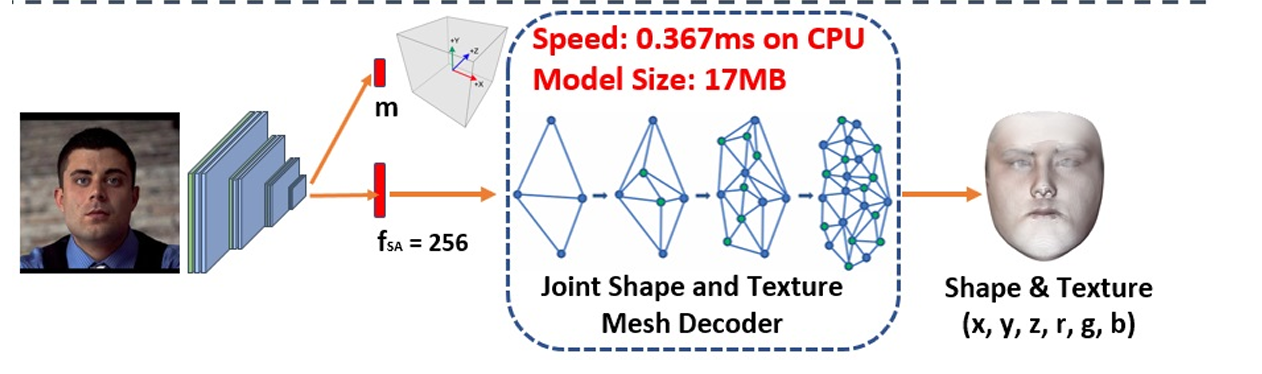
\includegraphics[width=1.1\textwidth]{meshdecoder.png}}
            \caption{Minh họa dataflow của mesh decoder mà paper lấy ý tưởng. Image sẽ được đưa qua feature pyramid để tạo ra các feature maps, tại Loss Head, một lớp 1 x 1 convolution layer dùng để trích xuất feature vector duy nhất cho mỗi anchor, từ vector này network predict ra các tham số chung cho cả texture và shape \(P_st \in \mathbb{R}^{128}\). Tiếp theo tham số được đưa qua Joint Mesh Decoder (sử dụng graph convolution) để tạo ra lưới \(V \in \mathbb{R}^{n \times 6}\) chứa cả Shape và Texture trên cùng một vertice.}
    \end{figure} 
    \item[+] Đồ thị Laplacian được định nghĩa \(\mathcal{L} = \mathcal{D} - \mathcal{E} \in \mathbb{R}^{n \times n}\) với \(\mathcal{D} \in \mathbb{R}^{n \times n}\) là ma trận đường chéo (diagonal matrix) với \(\mathcal{D}_{ii} = \sum_j\mathcal{E}_{ij}\)
    \item[+] Thông qua \cite{zhou2019dense,defferrard2016convolutional,ranjan2018generating}, graph convolution với kernel \(g_\theta\) có thể biểu diễn như recursive Chebyshev polynominal (đa thức Chebyshev đệ quy) được truncated ở bậc K
    \begin{equation}
        y = g_\theta(L)x = \sum_{k=0}^{K-1} \theta_k T_k(\tilde{L})x, \tag{2} 
    \end{equation}
    \item[+] Với \(\theta \in \mathbb{R}^K\) là vector của hệ số Chebyshev và \(T_k(\tilde{K} \in \mathbb{R}^{n \times n})\) là đa thức Chebyshev tại bậc k được evaluated tại scale Laplacian \(\tilde{L}\)
    \item[+] Với \(\bar{x} = T_k(\tilde{L})x \in \mathbb{R}^n\), ta có thể tính đệ quy \(\bar{x}_k = 2\tilde{K}\bar{x}_{k-1} - \bar{x}_{k - 2}\) với \(\bar{x}_0 = x \text{ và } \bar{x}_1 = \tilde{L}x\)
    \item[+] Toàn bộ quá trình lọc (filtering operation) cực kỳ hiệu quả bao gồm K tích ma trận thưa với một tích ma trận dày đặc \textbf{(dense matrix-vector)} \(y = g_\theta(L)x = [\bar{x}_0, \dots, \bar{x}_{k-1}]\theta \to \textbf{Fast  localised spectral filtering}\)
    \end{itemize}
    \item[--]\textbf{Differentiable Renderer:} Sau khi predict được shape và texture parameters \(P_{ST} \in \mathbb{R}^{128}\), nhóm tác giả đã sử dụng một bộ kết xuất lưới 3D khả vi (efficient differentiable 3D mesh renderer) để chiếu coloured-mesh (bộ lưới màu) \(\mathcal{D}_{P_{ST}}\) lên trên một mặt phẳng 2D image với các camera parameters \(P_{cam} = [x_c,y_c,z_c,x'_c,y'_c,z'_c,f_c]\) (camera location, camera pose và focal length (tiêu cực)) và illumination parameters (tham số ánh sáng | tham số chiếu sáng) \(P_{ill} = [x_l,y_l,z_l,r_l,g_l,b_l,r_a,g_a,b_a]\) (location of point light source (vị trí của điểm của nguồn sáng), colour values (giá trị màu) và colour of ambient lighting (màu sắc của ánh sáng môi trường)). 
    \item[--]\textbf{Dense Regression Loss:} Sau khi có được rendered 2D face \(\mathcal{R}(\mathcal{D}_{P_{ST}}, P_{cam}, P_{ill})\), ta sẽ tính toán sự khác biệt giữa pixel-wise của ảnh rendered và ảnh 2D gốc (được cắt ra từ anchor) sử dụng \(L_{pixel}\):
    \begin{equation}
    L_{pixel} = \frac{1}{W * H}\sum_{i}^{W}\sum_{j}^{H} \left\| \mathcal{R}(\mathcal{D}_{P_{ST}}, P_{cam}, P_{ill})_{i,j} - I_{i,j}^* \right\|_1 \tag{3}
    \end{equation}
    \begin{itemize}
        \item[+] Với W và H là width và height của anchor crop \(I_{i,j}^*\)
        \item[+] Anchor crop \(I_{i,j}^*\) chính là original 2D face được cắt ra (crop) từ anchor.
        \item[+] Hàm loss này sử dụng L1-norm để tính sai số tuyệt đối, sau đó chia trung bình cho tổng điểm số ảnh \((W * H)\)
        \item[+] L1-norm: Là tổng giá trị tuyệt đối của các phần tử trong vector (vector's components) \(\to\) Manhattan norm:
        \[\left\| x \right\|_1 = \sum_{i=1}^{n}|x_i|\]  
    \end{itemize}
\end{itemize}

\section{Implementation details:}
\begin{figure}[H]
    \makebox[\textwidth][c]{
        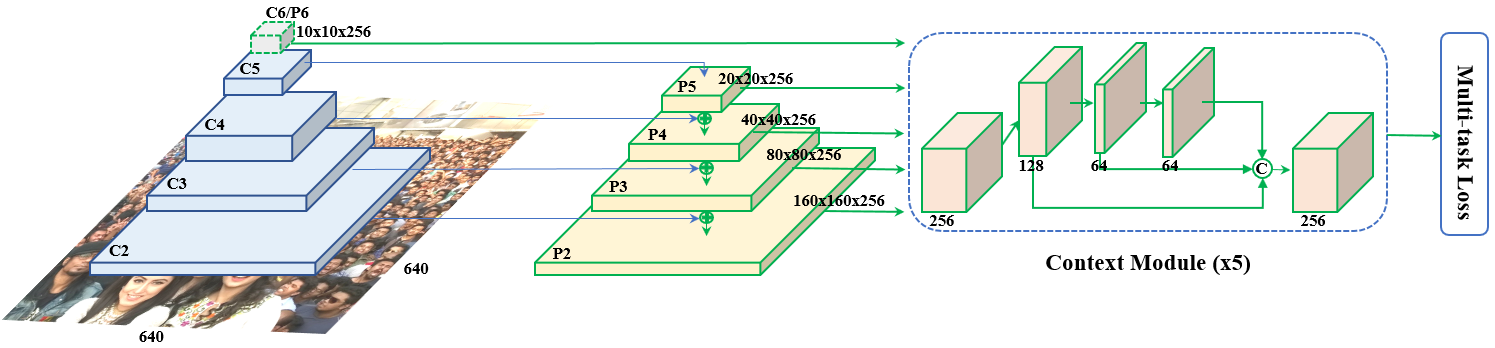
\includegraphics[width=1.3\textwidth]{framework.png}
    }
    \caption{Overview về phương pháp single-stage dense face localisation. RetinaFace được xây dựng dựa trên feature pyramids với những context module độc lập. Qua context modules, ta tính multi-task loss cho mỗi anchor}
\end{figure}
\subsection{Feature Pyramid}
\begin{itemize}
    \item[--] RetinaFace đã sử dụng feature pyramid levels từ \(P_2 \to P_6\), với \(P_2 \to P5\) được tính từ output (features map) tương ứng ResNet (Residual Network) \((C_2 \text{ đến } C_5)\) sử dụng top-down (kết nối từ trên xuống) và lateral connections (kết nối ngang).
    \item[--] \(P_6\) được tính thông qua 3 \(\times\) 3 convolution với stride = 2 trên \(C_5\)   
    \item[--] \(C_1 \to C_5\) sử dụng backbone là pre-trained ResNet-152 \cite{he2016deep} classification network trên bộ ImageNet-11K trong khi \(P_6\) được khởi tạo ngẫu nhiên bằng phương pháp "Xavier" \cite{glorot2010understanding}
\end{itemize}
\begin{enumerate}
    \item \textbf{Xavier method:}
    \begin{itemize}
        \item[+] Một phương pháp do nhóm tác giả của Xavier Glorot giới thiệu vào năm 2010.
        \item[+] Đây là phương pháp khởi tạo trọng số ban đầu (initial weights) cho các neural network.
        \item[+] Trong quá trình training deep neural network, nếu initial weights quá bé, dẫn đến \textbf{Vanishing Gradient}. Nếu initial weights quá lớn có thể dẫn đến \textbf{Exploding Gradient}. Xavier method được sinh ra nhằm giữ cho phương sai (variance) của các input và output variance ở mỗi lớp xấp xỉ bằng nhau, giúp các tín hiệu luân chuyển ổn định xuyên suốt network.
        \item[+] Trọng số \(W\) của một lớp neural sẽ được gán ngẫu nhiên bằng cách lấy mẫu từ một phân phối (thường là Uniform distribution (Phân phối đều) hoặc Normal distribution (Phân phối chuẩn)) có mean = 0 và variance được định nghĩa là:
        \item[+] \textbf{Uniform Xavier Initialization:}
        \begin{equation}
            x = \sqrt{\frac{6}{n_{inputs} + n_{outputs}}}
        \end{equation} 
        \begin{itemize}
            \item \(n_{inputs}\): Số lượng input của input layer
            \item \(n_{outputs}\): Số lượng output của output layer
            \item \(W\) sẽ được gán ngẫu nhiên trong uniform distribution giá trị nằm trong khoảng \([-x, x]\)
        \end{itemize}
        
        \item[+] \textbf{Normal Xavier Initialization}:  
        \[    \sigma = \sqrt{\frac{2}{n_{inputs} + n_{outputs}}} \]
        \begin{itemize}
            \item \(n_{inputs}\): Số lượng input của input layer
            \item \(n_{outputs}\): Số lượng output của output layer
            \item \(W\) sẽ được gán ngẫu nhiên trong normal distribution với mean = 0 và standard deviation (std) \(\sigma\)
        \[W \sim \mathcal{N}(0, \sigma^2) \]
        \end{itemize}
    \end{itemize}
    \item \textbf{ResNet:} \cite{he2016deep}
    \begin{itemize}
        \item[+] \textbf{ResNet (Residual Network)} được giới thiệu vào 2015 -- 2016, đây là một kiến trúc CNN.
        \item[+] Khi neural network có kiến trúc càng sâu (nhiều layer), hiện tượng Vanishing Gradient rất dễ xảy ra. ResNet sẽ giúp giải quyết vấn đề này bằng Residual Learning, bằng cách sử dụng các Residual Blocks kết hợp với Skip Connection, thay vì học trực tiếp hàm \(H(x)\), mạng học phần dư:
        \[F(x) = H(x) - x \quad ; \quad H(x) = F(x) + x\]  
        \item[+] Phần \(x\) được truyền trực tiếp qua skip connection, giúp gradient truyền tốt hơn trong backpropagation.
    \end{itemize}
    \begin{figure}[H]
        \makebox[\textwidth][c]{
            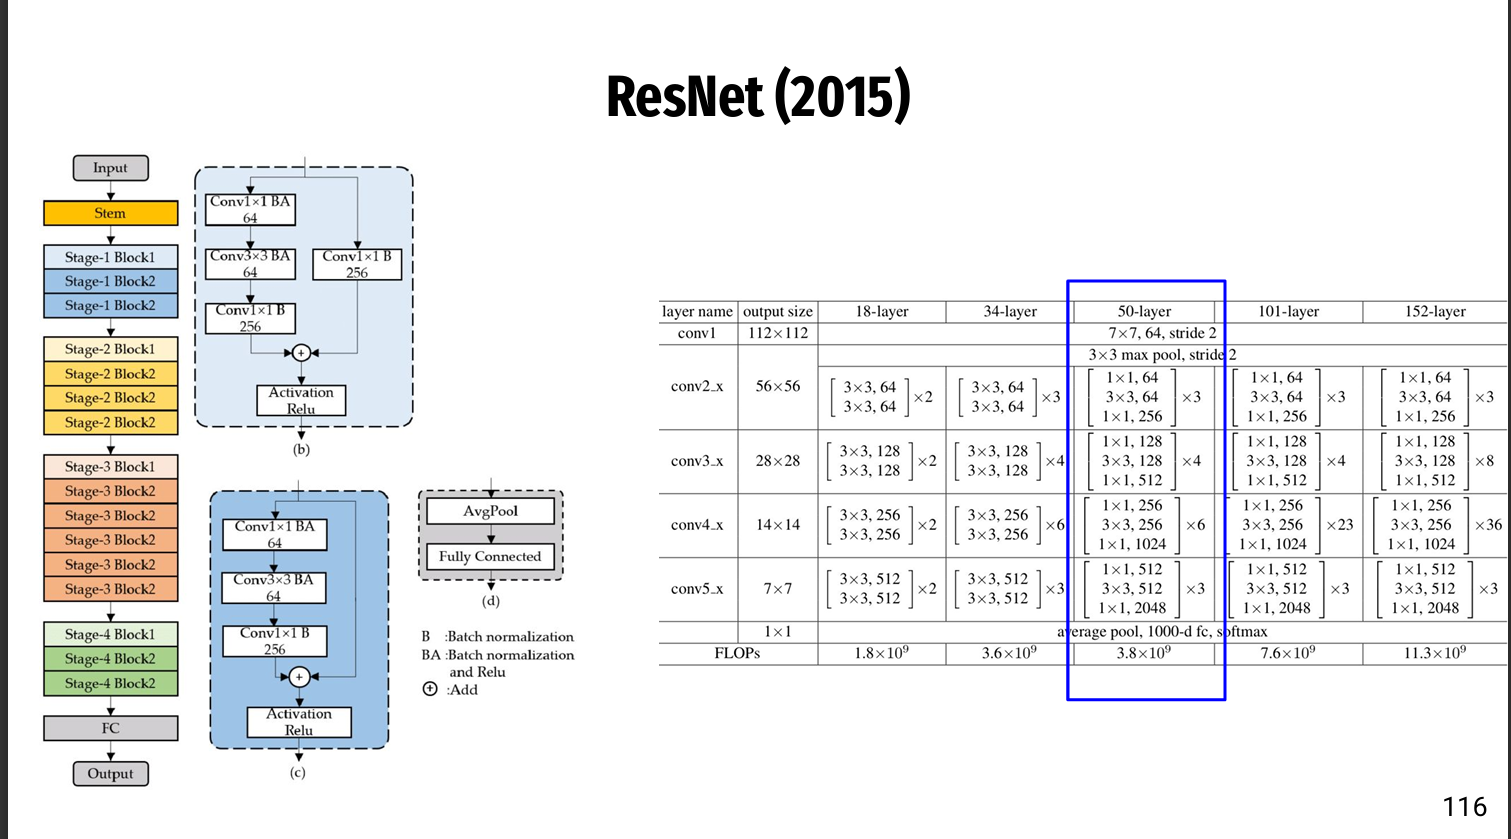
\includegraphics[width=1.3\textwidth]{ResNet.png}
        }
        \caption{Minh họa ResNet, ô được tô xanh là model ResNet50, ResNet152 là 152-layer bên phải.}
    \end{figure}
    \begin{figure}[H]
        \makebox[\textwidth][c]{
            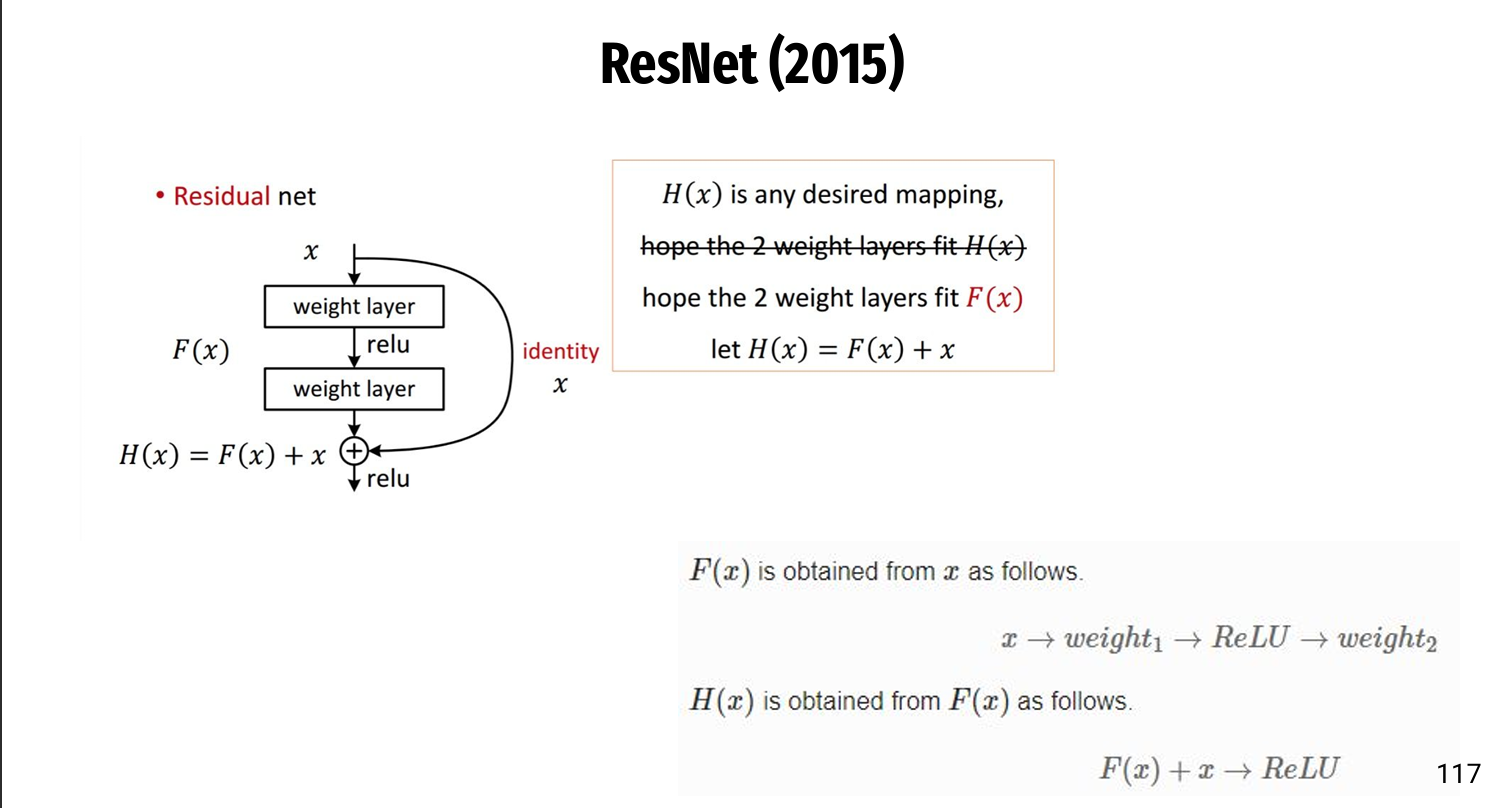
\includegraphics[width=1.3\textwidth]{ResidualNet.png}
        }
        \caption{Minh họa cách residual learning hoạt động}
    \end{figure}
\end{enumerate}
\subsection{Context Module:} \label{eq:context_modules}
\begin{itemize}
    \item[--] Được lấy cảm hứng từ SSH và PyramidBox, RetinaFace cũng áp dụng những context modules độc lập lên 5 tầng feature pyramid để mở rộng receptive field và tăng cường khả năng của rigid context modelling
    \item[--] Mô hình đã thay thế toàn bộ 3 \(\times\) 3 convolution layers bên trong lateral connection và context modules thành các deformable convolution network (DCN), giúp tăng cường non-rigid context modelling.
\end{itemize}
\begin{enumerate}
    \item \textbf{SSH và PyramidBox:}
    \begin{itemize}
        \item[+] \textbf{SSH (Single Stage Headless Face Detector):} 
        \begin{itemize}
            \item \textbf{Headless:} Kiến trúc này loại bỏ hoài toàn fully connected layers, giúp model nhẹ và nhanh hơn.
            \item \textbf{Context Module:} Thay vì dùng các filter có kích thước lớn (như 5 \(\times\) 5 hay 7 \(\times\) 7) tốn nhiều chi phí để mở rộng receptive field, SSH kết hợp song song các 3 \(\times\) 3 convolution layers. Việc stack hai lớp 3 \(\times\) 3 sẽ tạo hiệu ứng giống một lớp 5 \(\times\) 5, xếp chồng ba lớp 3 \(\times\) 3 tạo hiệu ứng 7 \(\times\) 7. Output của các nhanh này được concatenate lại với nhau, giúp network vừa nhẹ vừa bao quát được ngữ cảnh xung quanh khuôn mặt.
        \end{itemize}  
        \item[+] \textbf{PyramidBox (Context-assisted Single Shot Face Detector)}: Phức tạp hơn và chịu trách nhiệm xử lý các khuôn mặt bị che khuất hoặc tiny face, bao gồm:
        \begin{itemize}
            \item \textbf{Low-level Feature Pyramid Network}: Kết hợp thông tin từ nhiều layer của VGG16 network để tạo feature maps có độ phân giải cao, phù hợp cho tiny face.
            \item \textbf{CPM (Context-sensitive Predictor Module):} CPM predict thêm các bộ phận (đầu, vai, cơ thể) thay vì chỉ bounding box của khuôn mặt, giúp network có thể suy luận ra được vị trí khuôn mặt ngay cả khi bị mờ hoặc bị khuất.
        \end{itemize} 
    \end{itemize}
    \item \textbf{DCN (Deformable Convolutional Networks - Mạng tích chập biến dạng):} \cite{dai2017deformable}
    \begin{itemize}
        \item[+] Trong CNN cổ điển, các filter luôn sử dụng 3 \(\times\) 3 hay 5 \(\times\) 5. Tuy nhiên, trong thực tế khuôn mặt người có nhiều phức tạp (pose, emotion, \(\dots\)) khiến khả năng detect gặp nhiều hạn chế:
        \[y(p_0) = \sum_{p_n \in \mathcal{R}} w(p_n) \cdot x(p_0 + p_n)\] 
        \begin{itemize}
            \item Với \(\mathcal{R}\) là regular gird, là tập hợp các spatial locations xác định vị trí mà fitler "nhìn" vào để trích xuất dữ liệu trong feature map. Xác định receptive field size và dilation (độ giãn):
            \[\mathcal{R} = \{(-1, -1), (-1, 0), \dots, (0, 1), (1, 1)\}\] xác định một kernel 3 \(\times\) 3 với dilation 1
            \item \(w\) là trọng số của filter, \(x\) là giá trị pixel đầu vào và \(p_n\) là các vị trí cố định trên grid. Lưới này là cố định, do đó sẽ tiếp nhận cả pixel nhiễu ở background nếu object không có hình vuông.
        \end{itemize} 
        \item[+] DCN giúp giải quyết vấn đề trên. Cấu trúc của nó bao gồm 2 bước hoạt động song song: 
        \begin{itemize}
            \item \textbf{Nhánh học độ lệch (Offset Learning):} Feature map sẽ được đưa qua 1 lớp convolution để dự đoán các giá trị độ lệch \(\{\Delta p_n | n = 1,\dots,N\}\), với \(N = |\mathcal{R}|\). Các giá trị độ lệch này là số thực (ví dụ: lệch 1.5 pixel sang trái, 0.2 pixel xuống dưới).
            \item \textbf{Nhánh tích chập biến dạng (deformable convolution):} Convolution layer sẽ lấy mẫu ở vị trí đã được cộng thêm độ lệch thay vì lưới vuông cố định:
            \[y(p_0) = \sum_{p_n \in \mathcal{R}} w(p_n) \cdot x(p_0 + p_n + \Delta p_n)\]
            \item Vì vị trí mới \(p_0 + p_n + \Delta p_n\) thường là số thập phân và không nằm tròn trên một pixel cụ thể, DCN sử dụng bilinear interpolation (nội suy song tuyến tính) để tính toán giá trị tại điểm đó dựa trên 4 pixel gần nhất.
        \end{itemize}
        \begin{figure}[H]
        \makebox[\textwidth][c]{
            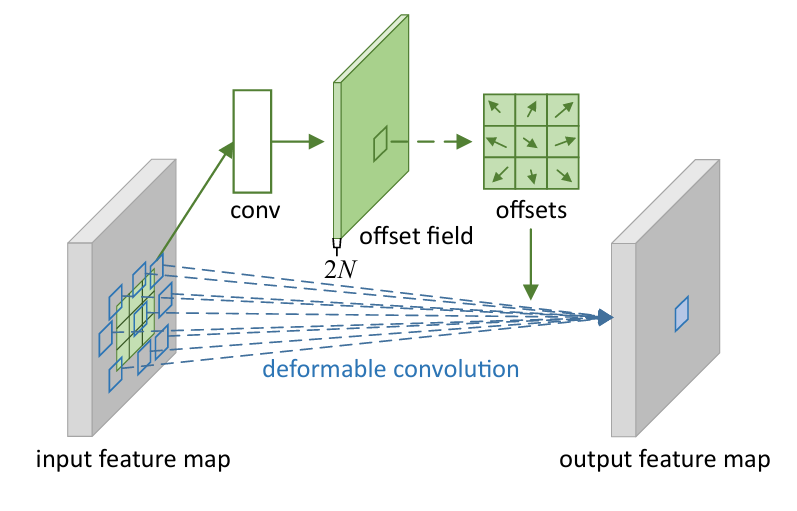
\includegraphics[width=1.1\textwidth]{DCN.png}
        }
        \caption{Minh họa 3 \(\times\) 3 deformable convolution.}
    \end{figure}
    \end{itemize} 
\end{enumerate}
\subsection{Loss Head:}
\begin{itemize}
    \item[--] Với negative anchors, chỉ áp dụng classification loss.
    \item[--] Với positive anchors, sử dụng multi-task loss.  
    \item[--] RetinaFace triển khai shared loss head (1 \(\times\) 1 conv) xuyên suốt feature maps ở các tầng khác nhau \(H_n \times W_n \times 256, n \in \{2,\dots,6\}\) (tương ứng với các tầng từ \(P_2 \to P_6\)).
    \item[--] Nhóm tác giả đã sử dụng pre-trained model \cite{zhou2019dense}, cho phép quá trình inference (suy luận) hiệu quả hơn nhưng chỉ tạo ra một lượng thụ phí tính toán nhỏ (small computational overhead).
\end{itemize}


\chapter{RetinaFace Source Code}
\section{Dataset:}
\begin{lstlisting}{language=Python, caption=Mã nguồn dataset}
        for label in labels:
            annotation = np.zeros((1, 15))
            # bbox (x1, x2, y1, y2)
            annotation[0, 0] = label[0] # x1
            annotation[0, 1] = label[1] # y1
            annotation[0, 2] = label[0] + label[2] # x1 + w -> x2
            annotation[0, 3] = label[1] + label[3] # y1 + h -> y2

            # Landmarks - With repo data format
            annotation[0, 4] = label[4]   # l0_x
            annotation[0, 5] = label[5]   # l0_y
            annotation[0, 6] = label[7]   # l1_x
            annotation[0, 7] = label[8]   # l1_y
            annotation[0, 8] = label[10]   # l2_x
            annotation[0, 9] = label[11]   # l2_y
            annotation[0, 10] = label[13] # l3_x
            annotation[0, 11] = label[14] # l3_y
            annotation[0, 12] = label[16] # l4_x
            annotation[0, 13] = label[17] # l4_y

            if label[4] >= 0:
                annotation[0, 14] = 1
            else:
                annotation[0, 14] = -1
\end{lstlisting}
\begin{itemize}
    \item[--] Điểm chú ý nhất của source code dataset chính là cách tạo \textbf{annotation:}
    \begin{itemize}
        \item[+] Mỗi face được lưu thành vector bao gồm các label được khởi tạo. Tổng cộng có 4 giá trị bounding box \((x_1, y_1, x_2, y_2)\), 10 landmark \((l_{0_x}, l_{0_y},\dots, l_{4_x}, l_{4_y})\) và một flag annotation[0, 14].
        \item[+] Label[6, 9, 12, 15] là vị trí của \textbf{visibility} và các giá trị này được bỏ qua.
        \item[+] Một face trong dataset có dạng:
        \begin{lstlisting}
    [x, y, w, h,
    l0_x, l0_y, v0,
    l1_x, l1_y, v1,
    l2_x, l2_y, v2,
    l3_x, l3_y, v3,
    l4_x, l4_y, v4]
        \end{lstlisting}
        \item[+] Trong đó:
        \begin{itemize}
            \item \((l_{0_x}, l_{0_y})\): left eye
            \item \(l_{1_x}, l_{1_y}\): right eye
            \item \(l_{2_x}, l_{2_y}\): nose 
            \item \(l_{3_x}, l_{3_y}\): left mouth
            \item \(l_{4_x}, l_{4_y}\): right mouth
        \end{itemize} 
        \item[+] Visibility flag annotation[0, 14] = 1: landmarks hợp lệ, annotation[0, 14] = -1: landmarks bị missing.
    \end{itemize} 
\end{itemize}
\section{Backbone:}
\begin{itemize}
    \item [--] Paper đã sử dụng ResNet làm backbone, để trích xuất đặc trưng tạo thành các feature maps trước khi được đưa qua Context Module
    \item [--] Tham khảo mã nguồn: \\
    \vspace{0.2cm}
    \url{https://github.com/yuuMQ/Retinaface_FaceDetection_Pytorch/blob/main/models/backbones/resnet.py}
    \begin{lstlisting}
        self.layer1 = self._make_layer(block, 64, layers[0])
        self.layer2 = self._make_layer(block, 128, layers[1], stride=2, dilate=replace_stride_with_dilation[0])
        self.layer3 = self._make_layer(block, 256, layers[2], stride=2, dilate=replace_stride_with_dilation[1])
        self.layer4 = self._make_layer(block, 512, layers[3], stride=2, dilate=replace_stride_with_dilation[2])

    \end{lstlisting}
    \item [--] Mỗi layer của ResNet là 1 Stage, trong đó chứa nhiều Residual Blocks.
    \item [--] Ví dụ quá trình forward:
    \begin{lstlisting}
        input x: (1, 3, 224, 224)
            1. conv1 -> bn -> relu -> maxpool
                output: (1, 64, 56, 56)
            2. Layer1:
                (1, 64 * expansion, 56, 56)
                - BasicBlock -> (1, 64, 56, 56)
                - Bottleneck -> (1, 256, 56, 56)
            3. Layer2:
                (1, 128 * expansion, 28, 28)
            4. Layer3:
                (1, 256 * expansion, 14, 14)
            5. Layer4:
                (1, 512 * expansion, 7, 7)
            6. AvgPool:
                (1, 512 * expansion, 1, 1)
            7. Flatten + Fc:
                (1, num_classes)
    \end{lstlisting}
    \newpage
    \item [--] Tổng số layers tương ứng với mỗi phiên bản Resnet:
    \begin{center}
        \begin{tabular}{|l|c|c|}
            \hline
            \textbf{Model} & \textbf{Layers (Số lượng block)} & \textbf{Tổng số Layers} \\
            \hline
            ResNet-18 & [2, 2, 2, 2] & 18 \\
            \hline
            ResNet-34 & [3, 4, 6, 3] & 32 \\
            \hline
            ResNet-50 & [3, 4, 6, 3] & 50 \\
            \hline
            ResNet-101 & [3, 4, 23, 3] & 101 \\
            \hline
            ResNet-152 & [3, 8, 36,, 3] & 152 \\
            \hline
        \end{tabular}
    \end{center}

\end{itemize}
\section{Layers:}
\begin{itemize}
    \item[--] \textbf{FPN (Feature Pyramid Network):}
    \begin{itemize}
        \item [+] FPN được triển khai cho multi-scale feature map extraction và mergin.
        \item [+] Sử dụng \textbf{1 \(\times\) 1 convolutions} cho output layers và \textbf{3 \(\times\) 3 convolutions} cho merging layers.
    \end{itemize}
    \begin{lstlisting}
    # 1x1 Convolution output layers
    self.output1 = Conv2dNormActivation(in_channels_list[0], out_channels, kernel_size=1, negative_slope=leaky)
    self.output2 = Conv2dNormActivation(in_channels_list[1], out_channels, kernel_size=1, negative_slope=leaky)
    self.output3 = Conv2dNormActivation(in_channels_list[2], out_channels, kernel_size=1, negative_slope=leaky)

    # Merge Layers with 3x3 Convolutions
    self.merge1 = Conv2dNormActivation(out_channels, out_channels, kernel_size=3, negative_slope=leaky)
    self.merge2 = Conv2dNormActivation(out_channels, out_channels, kernel_size=3, negative_slope=leaky)
    \end{lstlisting}
    \newpage
    \begin{itemize}
        \item[+] Quá trình forward:
    \end{itemize}
    \begin{lstlisting}
    '''
    :param inputs: input feature maps from diff levels of the pyramid
    :return: list of merged output feature maps at diff scales.
    '''

    inputs = list(inputs.values())

    # Apply output layers to each feature map
    output1 = self.output1(inputs[0])
    output2 = self.output2(inputs[1])
    output3 = self.output3(inputs[2])

    # Merge outputs with upsampling and addition
    upsample3 = F.interpolate(output3, size=output2.shape[2:], mode='nearest')
    output2 = self.merge2(output2 + upsample3)

    upsample2 = F.interpolate(output2, size=output1.shape[2:], mode='nearest')
    output1 = self.merge1(output1 + upsample2)

    return [output1, output2, output3]

    \end{lstlisting}
    \item[--] \textbf{SSH (Single Stage Headless):}
    \begin{itemize}
        \item [+] SSH module sử dụng cho feature extraction bằng cách kết hợp \(\{3 \times 3, 5 \times 5, 7 \times 7\}\) convolutions với batch normalization và activation function (LeakyReLU)
        \item [+] Thực chất đó là sự xếp chồng các convolution \(3 \times 3\) để mô phỏng \(5 \times 5, 7 \times 7 \) convolution layers, giúp cho network nhẹ hơn nhưng vẫn bao quát được không gian xung quanh khuôn mặt. 
    \end{itemize}
    \begin{lstlisting}
    # 3x3 Convolution branch
    self.conv3X3 = Conv2dNormActivation(in_channel, out_channel // 2, kernel_size=3, activation_layer=None)

    # 5x5 Convolution branch
    self.conv5X5_1 = Conv2dNormActivation(in_channel, out_channel // 4, kernel_size=3, negative_slope=leaky)
    self.conv5X5_2 = Conv2dNormActivation(out_channel // 4, out_channel // 4, kernel_size=3, activation_layer=None)

    # 7x7 Convolution branch
    self.conv7X7_2 = Conv2dNormActivation(out_channel // 4, out_channel // 4, kernel_size=3, negative_slope=leaky)
    self.conv7X7_3 = Conv2dNormActivation(out_channel // 4, out_channel // 4, kernel_size=3, activation_layer=None)  
    \end{lstlisting}
\end{itemize}
\section{Loss:}
\begin{itemize}
    \item[--] Với công thức Multi-task loss:
    \begin{equation}
    L = L_{cls}(p_i,p_i^*) + \lambda_1p_i^*L_{box}(t_i,t_i^*) + \lambda_2p_i^*L_{pts}(l_i,l_i^*) + \lambda_3p_i^*L_{pixel}.
    \end{equation}
    ta có:
    \begin{itemize}
        \item[+] \(L_{cls}\): Classification Loss \(L_{conf}\)
        \item[+] \(L_{box}\): Face box regression Loss, trong source code, loss này được tính dựa trên sai số tọa độ của bounding box, được gọi là \textbf{Localization Loss} \(L_{loc}\)
        \item[+] \(L_{pts}\): Facial landmark regression Loss \(F_{landm}\), sai số của 5 facial feature tương ứng với 10 tọa độ \((x, y)\)
    \end{itemize}
    \newpage
    \begin{lstlisting}
    # Landmark Loss (Smooth L1)
    landm_p = landmark_preds[pos_idx1].view(-1, 10)
    lnm_targets = lnm_targets[pos_idx1].view(-1, 10)
    loss_landm = F.smooth_l1_loss(landm_p, lnm_targets, reduction='sum')
    \end{lstlisting}
    \begin{lstlisting}
    # Localization Loss (Smooth L1)
    pos_idx = pos_mask.unsqueeze(pos_mask.dim()).expand_as(loc_preds)
    loc_p = loc_preds[pos_idx].view(-1, 4)
    loc_targets = loc_targets[pos_idx].view(-1, 4)
    loc_loss = F.smooth_l1_loss(loc_p, loc_targets, reduction='sum')
    \end{lstlisting}
    \begin{lstlisting}
    # Confidence Loss Including Positive and Negative Examples
    pos_idx = pos_mask.unsqueeze(2).expand_as(conf_preds)
    neg_idx = neg_mask.unsqueeze(2).expand_as(conf_preds)
    conf_p = conf_preds[(pos_idx + neg_idx).gt(0)].view(-1, num_classes)
    targets_weighted = conf_targets[(pos_mask+neg_mask).gt(0)]
    conf_loss = F.cross_entropy(conf_p, targets_weighted, reduction='sum')
    \end{lstlisting}
    \begin{lstlisting}
# Sum of losses: L(x,c,l,g) = (Lconf(x, c) + αLloc(x,l,g)) / N
    N = max(num_pos.sum().float(), 1)
    loc_loss /= N
    conf_loss /= N
    loss_landm /= N1

    return loc_loss, conf_loss, loss_landm
    \end{lstlisting}
\end{itemize}
\section{Optimizer:}
\begin{itemize}
    \item[--] RetinaFace sử dụng SGD \textbf{(Stochastic Gradient Descent)} Optimizer:
    \begin{equation}
        \theta = \theta - \eta \nabla_\theta J(\theta; x_i,y_i)
    \end{equation} 
    \item[--] Sự khác biệt giữa \textbf{Gradient Descent} và \textbf{Stochastic Gradient Descent}
\end{itemize}

\begin{center}
    \renewcommand{\arraystretch}{2.5} % Tăng khoảng cách dòng để công thức không chạm dòng kẻ
    \begin{tabularx}{\textwidth}{|l|X|X|} % \textwidth giúp bảng dàn hàng ngang hết cỡ
        \hline
        & \centering \textbf{Gradient Descent} & \centering \textbf{Stochastic Gradient Descent} \tabularnewline
        \hline
        \textbf{Công thức} & 
        \centering $\theta = \theta - \eta \cdot \frac{1}{n} \sum_{i=1}^{n} \nabla_{\theta} J_i(\theta)$ & 
        \centering $\theta = \theta - \eta \cdot \nabla_{\theta} J_i(\theta)$ \tabularnewline
        \hline
        \textbf{Dữ liệu mỗi step} & Sử dụng \textbf{toàn bộ} tập huấn luyện ($n$ mẫu). & Sử dụng duy nhất \textbf{1 mẫu} dữ liệu ngẫu nhiên. \tabularnewline
        \hline
        \textbf{Tốc độ hội tụ} & Chậm (do phải tính toán trên toàn bộ tập dữ liệu). & Nhanh (cập nhật ngay lập tức sau mỗi mẫu). \tabularnewline
        \hline
        \textbf{Đường tối ưu} & Mượt mà, đi thẳng đến cực tiểu. & Zic-zac, dao động mạnh xung quanh cực tiểu. \tabularnewline
        \hline
        \textbf{Thoát Local Minimum} & Kém, dễ bị kẹt tại các hố nông. & Tốt hơn nhờ sự dao động (nhiễu) giúp nhảy khỏi hố. \tabularnewline
        \hline
    \end{tabularx}
\end{center}

\section{Model:}
\begin{itemize}
    \item[--] Sử dụng backbone (ResNet) để trích xuất đặc trưng (feature extraction).
    \item[--] FPN: Kết hợp thông tin ngữ nghĩa từ các deep layer với thông tin không gian từ shallow layer.
    \item[--] SSH: Tăng cường receptive field thông qua các convolution layer xếp chồng.
    \item[--] Multi-task Heads: Thực hiện dự đoán song song trên các feature maps.  
\begin{lstlisting}
    backbone = build_backbone(cfg['name'], cfg['pretrain'])
    self.fx = get_layer_extractor(cfg, backbone) # feature extraction

    num_anchors = 2
    base_in_channels = cfg['in_channel']
    out_channels = cfg['out_channel']

    fpn_in_channels = [
        base_in_channels * 2,
        base_in_channels * 4,
        base_in_channels * 8,
    ]

    self.fpn = FPN(fpn_in_channels, out_channels)
    self.ssh1 = SSH(out_channels, out_channels)
    self.ssh2 = SSH(out_channels, out_channels)
    self.ssh3 = SSH(out_channels, out_channels)

    self.class_head = ClassHead(in_channels=cfg['out_channel'], num_anchors=num_anchors, fpn_num=3)
    self.bbox_head = BboxHead(in_channels=cfg['out_channel'], num_anchors=num_anchors, fpn_num=3)
    self.landmark_head = LandmarkHead(in_channels=cfg['out_channel'], num_anchors=num_anchors, fpn_num=3)
\end{lstlisting}
\newpage
    \item[--] Quá trình forward:
\begin{lstlisting}
    out = self.fx(x)
    fpn = self.fpn(out)

    # single-stage headless module
    feature1 = self.ssh1(fpn[0])
    feature2 = self.ssh2(fpn[1])
    feature3 = self.ssh3(fpn[2])

    features = [feature1, feature2, feature3]

    classifications = self.class_head(features)
    bbox_regressions = self.bbox_head(features)
    landmark_regressions = self.landmark_head(features)

    if self.training:
        output = (bbox_regressions, classifications, landmark_regressions)
    else:
        output = (bbox_regressions, F.softmax(classifications, dim=-1), landmark_regressions)
    return output
\end{lstlisting}
\end{itemize}

\chapter{Ý tưởng cải tiến:}
\section{Hạn chế của paper hiện tại:}
\section{Swin Transformer for feature extraction:}
\section{Feature Enhancement Feature Pyramid Network:}


\chapter{Kết quả thực nghiệm:}
Kết quả trên \textbf{WiderFace Evaluation Set} theo báo cáo của repository

\begin{itemize}
    \item[--] Multi-scale image resizing:
    \begin{center}
    \begin{tabular}{|l|c|c|c|c|}
        \hline
        \textbf{RetinaFace Backbones} & \textbf{Easy} & \textbf{Medium} & \textbf{Hard} \\
        \hline
        MobileNetV1 & 90.59\% & 89.14\% & 84.13\% \\
        \hline
        MoblieNetV2 & 91.70\% & 91.03\% & 86.60\% \\
        \hline
        ResNet18 & 92.50\% & 91.02\% & 86.63\% \\
        \hline
        ResNet34 & 94.16\% & 93.12\% & 88.90\% \\
        \hline  
    \end{tabular}
    \end{center} 
    \item[--] Original image size:  
    \begin{center}
    \begin{tabular}{|l|c|c|c|c|}
        \hline
        \textbf{RetinaFace Backbones} & \textbf{Easy} & \textbf{Medium} & \textbf{Hard} \\
        \hline
        MobileNetV1 & 92.19\% & 90.41\% & 79.56\% \\
        \hline
        MoblieNetV2 & 94.04\% & 92.26\% & 83.59\% \\
        \hline
        ResNet18 & 94.28\% & 92.69\% & 82.95\% \\
        \hline
        ResNet34 & 95.07\% & 93.48\% & 84.40\% \\
        \hline  
    \end{tabular}
    \end{center}
\end{itemize}



\chapter{Kết luận}


\newpage
\bibliographystyle{ieeetr}
\bibliography{tailieu}

\end{document}
